\documentclass[10pt,a4paper,titlepage]{article}
\usepackage[utf8]{inputenc}
\usepackage[german]{babel}
\usepackage{amsmath}
\DeclareMathOperator{\arcsec}{arcsec}
\usepackage{amsfonts}
\usepackage{amssymb}
\usepackage[affil-it]{authblk}
\usepackage{graphicx}
\graphicspath{{images/}}
\usepackage{hyperref}
\usepackage{siunitx}
\usepackage{cite}
\usepackage{xcolor}
\newcommand{\highlight}[1]{\colorbox{red!50}{$\displaystyle#1$}}
\usepackage[nottoc,numbib]{tocbibind}
\begin{document}
\begin{titlepage}
\author[1]{Sven Seeberg}
\affil[1]{Sternwarte Regensburg}
\title{Astrofotografie-Praktikum der Volkssternwarte Regensburg}
\end{titlepage}
\maketitle

\tableofcontents
\section{Lizenz}
Diese Anleitung ist lizenziert mit einer \textit{Creative Commons Attribution-ShareAlike 4.0 International Lizenz}. Eine Kopie der Lizenz ist hier verfügbar: \url{https://creativecommons.org/licenses/by-sa/4.0/deed.de}.

Einige der hier verwendeten Bilder stehen unter anderen Lizenzen. Dies ist beim jeweiligen Bild vermerkt.


\section{Einleitung}
An der Sternwarte Regensburg können die verschiedenen Methoden zur Erfassung und Verarbeitung astronomischer Bilddaten ausprobiert werden. Neben qualitativ hochwertigen Teleskopen verschiedenster Bauweisen stehen Kameras speziell für astronomische Zwecke zur Verfügung. Mit ihnen können sowohl Planeten- als auch Deep-Sky-Bilder, sowie Spektren aufgenommen werden. In der folgenden Anleitung sind die theoretischen Grundlagen und die praktische Durchführung der Aufnahmemethoden geschildert.

Ein großer Teil der zur Bearbeitung benötigten Programme ist kostenlos im Internet erhältlich. Die Links sind jeweils angegeben. Es wird empfohlen einen eigenen Laptop mitzubringen, um die in großen Mengen anfallenden Daten dort speichern zu können. Gegebenenfalls können die Daten dann zu Hause fertig bearbeitet und ausgewertet werden.
\section{Teleskope}
Die Sternwarte Regensburg hat Teleskope verschiedenster Bauart zur Verfügung. In der Kuppel befinden sich ein \href{https://de.wikipedia.org/wiki/Apochromat}{Apochromatischer Refraktor} (6'' Durchmesser, sprich 6 Zoll, $1\dq = \SI{2,54}{cm}$), sowie ein \href{https://de.wikipedia.org/wiki/Cassegrain-Teleskop}{Cassegrain-Teleskop} (12,5''). Auf der Plattform befinden sich fest montiert ein 11'' und ein 12'' \href{https://de.wikipedia.org/wiki/Schmidt-Cassegrain-Teleskop}{Schmidt-Cassegrain-Teleskop}. Weiter zur Verfügung stehen verschiedene \href{https://de.wikipedia.org/wiki/Newton-Teleskop}{Newton-Teleskope}, sowie \href{https://de.wikipedia.org/wiki/H-alpha-Teleskop}{Sonnenteleskope mit H-Alpha-Filtern}. [Für Details zu den Bauweisen sei auf die Wikipedia-Artikel verwiesen.]
Wir vernachlässigen im Folgenden die unterschiedlichen Bauweisen und betrachten das Linsenteleskop etwas näher. Die primäre Aufgabe eines Teleskops ist das Sammeln und Bündeln von Licht. Das Lichtsammelvermögen eines Teleskops steigt mit der Öffnungsfläche $A$, das heißt dem Quadrat des Öffnungsradiuses $r$. Bei Teleskopen wird in der Regel der Durchmesser $D = 2 \cdot r$ angegeben.
\begin{equation}
A = \pi r^2 = \pi \biggr ( \frac{D}{2} \biggr )^2
\end{equation}

\subsection{Auflösungsvermögen}
\begin{figure}[h!]
  \centering
    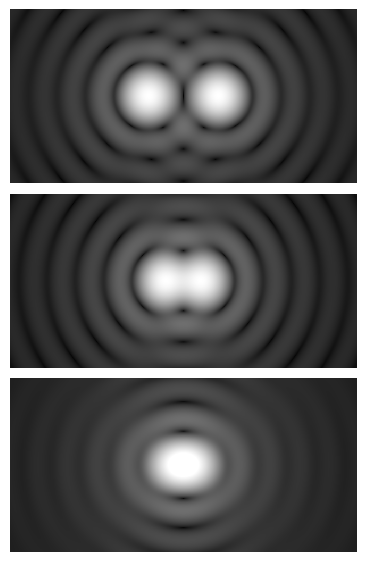
\includegraphics[width=0.4\textwidth]{Airy_disk}
  \caption{Beugungsscheibchen einer runden Öffnung mit unterschiedlichen Abständen. Quelle: \url{https://en.wikipedia.org/wiki/File:Airy_disk_spacing_near_Rayleigh_criterion.png}}
  \label{fig:aufloesung}
\end{figure}
Ebenfalls abhängig vom Teleskopdurchmesser ist das so genannte Auflösungs-vermögen. Das bedeutet, dass zwei eng beisammen liegende Lichtquellen erst ab einem hinreichend großen Teleskopdurchmesser als zwei getrennte Objekte identifiziert werden könnten (\textit{Abbildung \ref{fig:aufloesung}}). Neben dem Durchmesser ist das Auflösungsvermögen zusätzlich von der Wellenlänge des Lichts abhängig. Da Licht seiner Natur nach als elektromagnetische Welle beschrieben werden kann, kann man den Farben des Lichts Wellenlängen zuordnen. Blaues Licht hat dabei eine Wellenlänge von ungefähr $\lambda = 450 nm$, rotes Licht hat eine Wellenlänge von ungefähr $\lambda = 620 nm$. Das Auflösungsvermögen wird in einem Winkel $\delta_{min}$ angegeben, unter dem zwei Objekte gerade noch zu trennen sind. Konkret gibt $\delta_{min}$ den Radius des Beugungsscheibchens an, welches durch Interferenz der Lichtwellen an einer runden Öffnung hervorgerufen wird.
\begin{equation}
\delta_{min} = \sin^{-1}\biggr(1,22 \frac{\lambda}{D}\biggr)
\end{equation}
Dementsprechend ist das Auflösungsvermögen des selben Teleskops für blaues Licht besser als für rotes Licht (unterschiedliche Wellenlängen für $\lambda$ einsetzen!). Für Teleskope jenseits einer Öffnung von 8'' ist allerdings nicht mehr das Auflösungsvermögen des Teleskops der limitierende Faktor, sondern die Erdatmosphäre. Ursache sind unterschiedliche Temperaturen in den Luftschichten, die unterschiedliche Luftdichten zur Konsequenz haben, da der Brechungsindex eines Gases von dessen Dichte abhängt. Dadurch wird Licht in der Atmosphäre immer vielfach gebrochen. Dazu kommen Bewegungen der Luftschichten, die dazu führen, dass sich die Brechung des Lichts kontinuierlich ändert. Dieses Phänomen nennt man Seeing und führt dazu, dass selbst unter idealen Bedingungen das Auflösungsvermögen nie besser als \ang{;;1} ist.
\subsection{Abbildung}
\label{sec:abbildung}
\begin{figure}[h!]
  \centering
    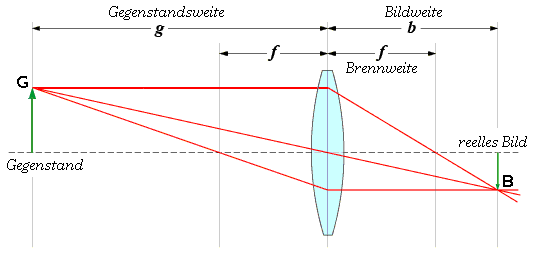
\includegraphics[width=0.75\textwidth]{Sammellinse}
  \caption{Abbildung mit einer Sammellinse. Quelle: \url{https://de.wikipedia.org/wiki/Datei:Sammellinse_Skizze.png}, Lizenz: \href{http://www.selflinux.org/selflinux/html/gfdl_de.html}{GFDL}}
  \label{fig:sammellinse}
\end{figure}
Die Primäroptik eines Teleskops (Linse oder Spiegel) bündelt (annähernd parallele) Strahlen von einfallendem Licht im Brennpunkt. Wird ein Gegenstand (Planet) angeschaut, entsteht ein Bild des Gegenstands in der Brennebene (Fläche mit dem Abstand der Brennweite von der Linse). Hielte man nun ein Blatt Papier in die Brennebene, könnte man das Abbild des Planeten mit dem Auge betrachten. Die Größe des Bildes $B$ ist dabei gegeben durch
\begin{equation}
\label{eq:bildgroesse}
B = G \cdot \frac{b}{g}
\end{equation}
Für die Beziehung von Brenn-, Gegenstands- und Bildweite gilt
\begin{equation}
\frac{1}{f} = \frac{1}{b}+\frac{1}{g}
\end{equation}
Bei sehr weit entfernten Objekte wird der Summand $\frac{1}{g}$ sehr klein und kann vernachlässigt werden. Daher gilt dann für die Brennweite
\begin{equation}
\label{eq:b-f}
\frac{1}{f} \approx \frac{1}{b}
\end{equation}
Die Brennweite des Teleskops, sowie die Gegenstandsgröße und -Abstand sind bekannt (\textit{Tabellen \ref{stw-teleskope} und \ref{planeten}}). Die Bildgröße hängt also linear von der Gegenstandsgröße, dem Gegenstandsabstand, sowie von der Brennweite ab. Die Größenordnung der Bildgröße der Planeten beträgt bei den Teleskopen der Sternwarte Regensburg ungefähr \SI{0.5}{\mm}.

\begin{table}
\begin{center}
\begin{tabular}{|c|c|c|}
\hline
\emph{Teleskop} & $f$ [mm] & $D$ [mm] \\
\hline
Kuppel-Refraktor & 2250 & 150 \\
Kuppel-Cassegrain & 4750 & 317,5 \\
Meade 12" & 3000 & 304 \\
Celestron 11" & 2800 & 280 \\
\hline
\end{tabular}
\caption{Brennweiten und Durchmesser der Teleskope der Sternwarte}
\label{stw-teleskope}
\end{center}
\end{table}

\begin{table}
\begin{center}
\begin{tabular}{|c|c|c|c|}
\hline
\emph{Planet} & Durchmesser [km] & Minimalabstand [km] & Maximalabstand [km] \\
\hline
Mars & 6800 & 55 650 000 & 399 580 000 \\
Jupiter & 140 000 & 591 970 000 & 965 520 000 \\
Saturn & 116 000 & 1 204 280 000 & 1 652 480 000\\
\hline
\end{tabular}
\caption{Abstände und Durchmesser der Planeten}
\label{planeten}
\end{center}
\end{table}

\section{Grundlagen der Fotografie}
\subsection{Spektrum des Lichts}
Falls nur der Versuchsteil \textit{Planetenfotografie} durchgeführt wird, kann dieser Abschnitt übersprungen werden. Als Einleitung für das Thema Spektroskopie werden folgende Artikel zur Einführung empfohlen:
\begin{itemize}
\item \url{https://de.wikipedia.org/wiki/Licht}
\item \url{https://de.wikipedia.org/wiki/Spektrallinie}
\item \url{https://de.wikipedia.org/wiki/Astrospektroskopie}
\end{itemize}

\subsection{Farbbilder}
Bilder werden auf Computern in Form einer Sammlung von rechteckig angeordneten Pixeln, welche \href{https://de.wikipedia.org/wiki/Rastergrafik}{kleinste Bildeinheiten} sind, dargestellt. In den einfachsten Bildformaten, wir nehmen hier die \href{https://de.wikipedia.org/wiki/Windows_Bitmap}{Bitmap}, trägt jedes Pixel für seine Fläche eine Farb- und Helligkeitsinformation. Der Farb- und Helligkeitswert wird beispielsweise als Rot-Grün-Blau-Wert (RGB) gespeichert. Für jede der drei genannten Farben gibt es dann einen Helligkeitswert zwischen 0 und 255. Durch die Kombination der drei Farben können dann insgesamt bis 16 Millionen verschiedene Farben dargestellt werden. Sind die drei RGB-Werte genau gleich, handelt es sich um eine Graufstufe, dabei ist (0, 0, 0) Schwarz und (255, 255, 255) Weiß. Der Farbwert (255, 0, 0) ist dann beispielsweise die Farbe Rot. Zur Speicherung von 256 verschiedenen Kombinationen benötigt man am Computer genau 1 Byte, das heißt 8 Bit. 1 Bit kann dabei nach dem Binärsystem immer entweder 0 oder 1 sein. Sofern es 256 Farbwerte pro Farbkanal gibt, spricht man von einer so genannten Farbtiefe von 8 Bit. Um Bildinformationen von Licht an den PC zu übertragen, werden CCD- oder CMOS-Fotosensoren genutzt.
\begin{figure}[h!]
  \centering
    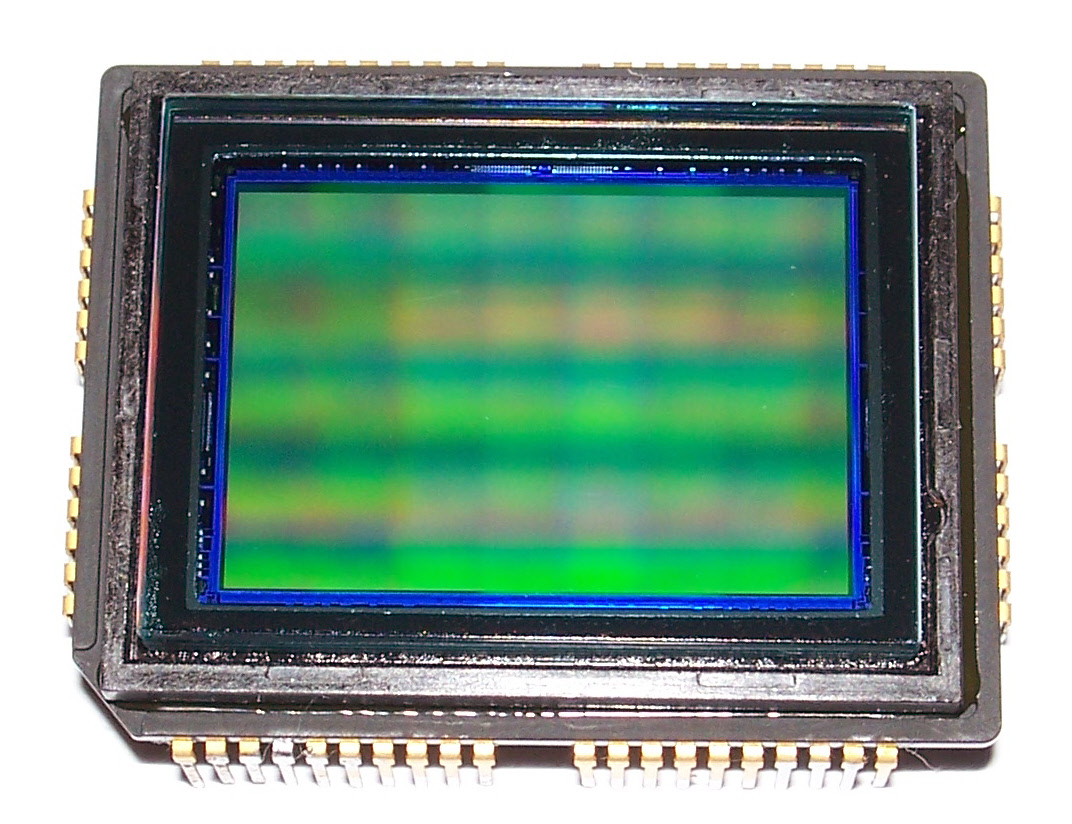
\includegraphics[width=0.5\textwidth]{Sony-CCD-Sensor}
  \caption{Ein CCD-Sensor von Sony. Quelle: \url{https://commons.wikimedia.org/wiki/File:CCD_SONY_ICX493AQA_sensor_side.jpg}, Lizenz: \href{https://creativecommons.org/licenses/by-sa/4.0/deed.en}{CC-BY-SA 4.0}}
  \label{fig:sony-ccd}
\end{figure}
Fotosensoren bestehen aus in einem Raster angeordneten Pixeln, die einfallendes Licht (Photonen) in ein elektrisches Signal umwandeln. Die einzelnen Pixel können nicht unterscheiden, welche Farbe ein einfallendes Photon hat, es handelt sich also zunächst um ein Schwarz-Weiß-Bild. Man schafft dadurch Abhilfe, dass man vor die Pixel Farbfilter legt.
\begin{figure}[h!]
  \centering
    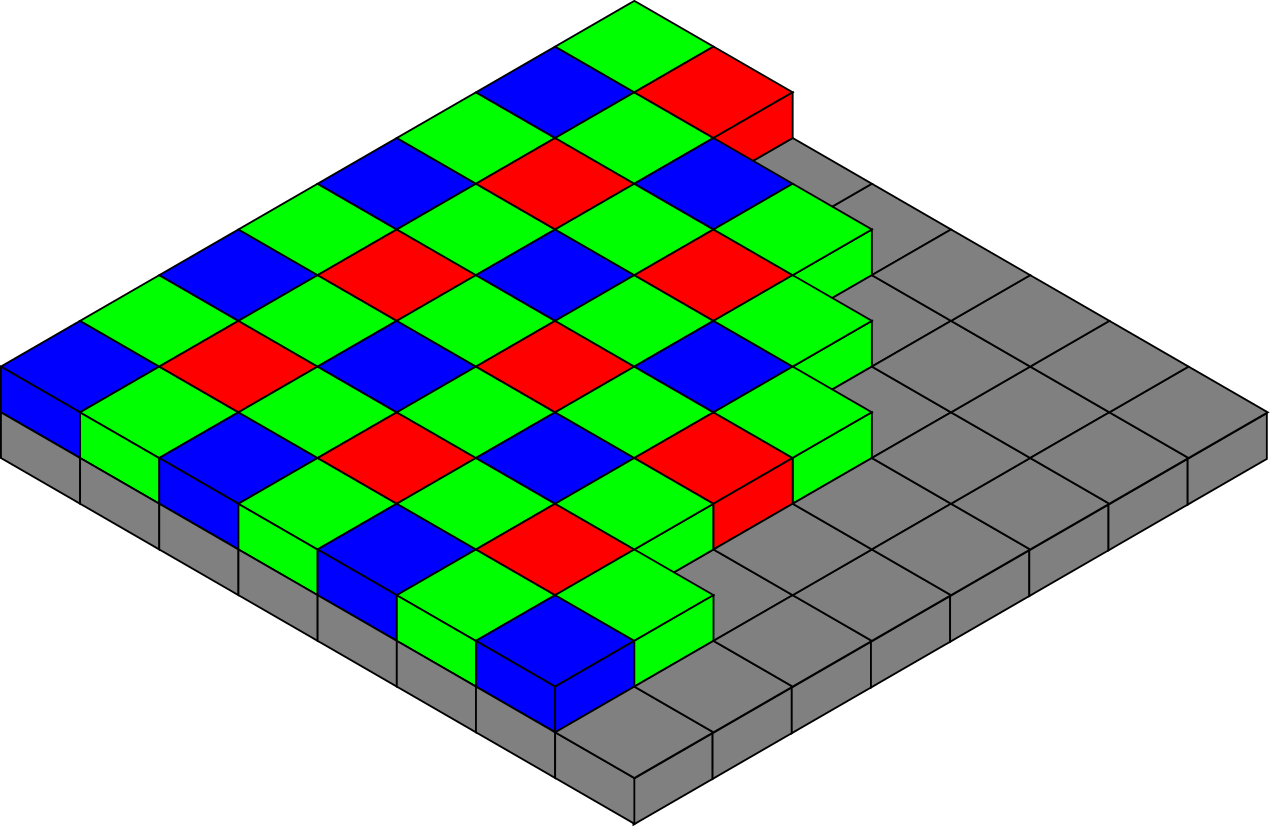
\includegraphics[width=0.75\textwidth]{Bayer-Matrix}
  \caption{Pixel eines CMOS- oder CCD-Sensors mit darübergelegtem Farbfilter. Die Anordnung von 2 Grün-Filtern, und jeweils einem Rot- und Blau-Filter pro 4 Pixel nennt man Bayer-Matrix. Quelle: \url{https://en.wikipedia.org/wiki/File:Bayer_pattern_on_sensor.svg}, Lizenz: \href{http://www.selflinux.org/selflinux/html/gfdl_de.html}{GFDL}}
  \label{fig:bayermatrix}
\end{figure}
Das hat zur Folge, dass in die Pixel entweder nur rote, grüne oder blaue Photonen fallen. Eine Möglichkeit, Farbfilter anzuordnen, ist die Bayer-Matrix (\textit{Abbildung \ref{fig:bayermatrix}}). Die Informationen von jeweils zwei grünen, einem roten und einem blauen Pixel werden zu einem RGB-Wert für ein Pixel zusammengefasst. Der Nachteil eines Bayermatrix-Farbfilters ist, dass der Farbfilter einen großen Teil der einfallenden Photonen herausfiltert, das heißt man verschenkt Helligkeit und Auflösungsvermögen. Für astronomische Zwecke ist das ungeschickt, da so Bildinformationen verloren gehen. In der Astronomie setzt man daher in zeitlicher Folge verschiedene Farbfilter vor den kompletten Sensor. Man erstellt also beispielsweise drei Schwarz-Weiß-Bilder mit abwechselnd einem Rot-, Grün- und Blau-Filter. Aus den 3 Bildern lässt sich dann ebenfalls wieder leicht ein RGB-Bild zusammensetzen.

\noindent\fbox{\parbox{\textwidth}{\textbf{Anmerkung:} Es können auch andere Farbfilter eingesetzt werden, beispielsweise Schmalband-Filter, die nur Licht mit ganz bestimmten Wellenlängen durchlassen. Das kann genutzt werden, um gezielt Licht von bestimmten Gasen (Wasserstoff, Sauerstoff, etc.) herauszufiltern und aufzunehmen. Mit dieser Technik werden Fotos von Deep-Sky-Objekten (Gasnebel und Galaxien) aufgenommen.

Außerdem werden in der Astrofotografie in der Regel Kameras mit einer Farbtiefe von mehr als 8 Bit eingesetzt, beispielsweise 10 oder 12 Bit. Das ermöglicht das Erfassen größerer Helligkeitsunterschiede. Diese Informationen müssen dann in anderen Bildddateien, üblicherweise FITS oder TIFF, gespeichert werden. Wir benutzen in diesem Praktikum allerdings Bitmaps, da diese mit allen üblichen Programmen geöffnet und bearbeitet werden können.}}

\subsection{Rauschen}
Jedes Pixel einer Kamera kann als eine Art Helligkeits- oder Lichttopf verstanden werden. Je nach Farbtiefe der Kamera, die in der Regel 8 Bit beträgt, aber bei astronomischen Kameras auch 10 Bit sein kann, hat der Lichttopf also 256, 512 oder 1024 diskrete Helligkeitswerte. Je länger Licht auf den Lichtsensor fällt, desto stärker werden die Lichttöpfe gefüllt, abhängig von der Helligkeit des beobachteten Objekts.

Natürlich sind auch Fotosensoren nicht perfekt, und beim Sammeln der Photonen und Auslesen der Daten passieren Fehler. Diese Fehler führen dazu, dass die real ausgelesenen Helligkeitswerte von den theoretischen Helligkeiten abweichen. Diese Abweichungen sind weitgehend zufällig und schwanken um den Helligkeit, den ein Pixel haben sollte. Man nennt diese Helligkeitsschwannkungen Rauschen. Das Rauschen ist weitgehend unabhängig von der Helligkeit eines Pixels. Bei geringen Helligkeiten ist die durch das Rauschen bedingte relative Helligkeitsschwankung also größer als bei größeren Helligkeiten.

\begin{figure}[h!]
  \centering
    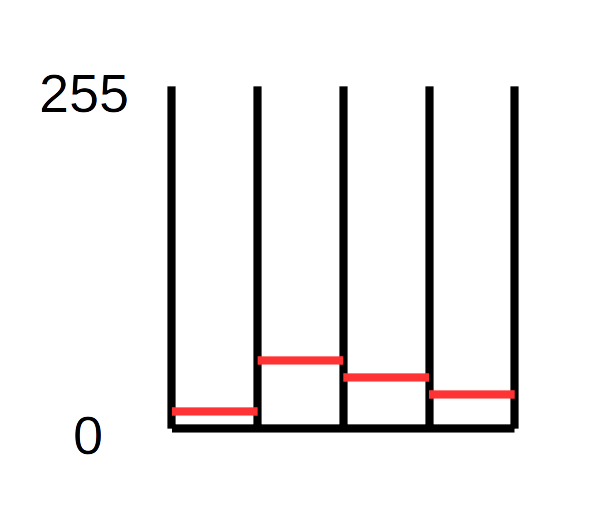
\includegraphics[width=0.5\textwidth]{CCD_geringe_Helligkeit}
  \caption{Helligkeitsverteilung über 4 Pixel bei geringer Helligkeit. In absoluten Zahlen unterscheiden sich die Helligkeiten nur wenig.}
  \label{fig:ccd-dunkel}
\end{figure}

\begin{figure}[h!]
  \centering
    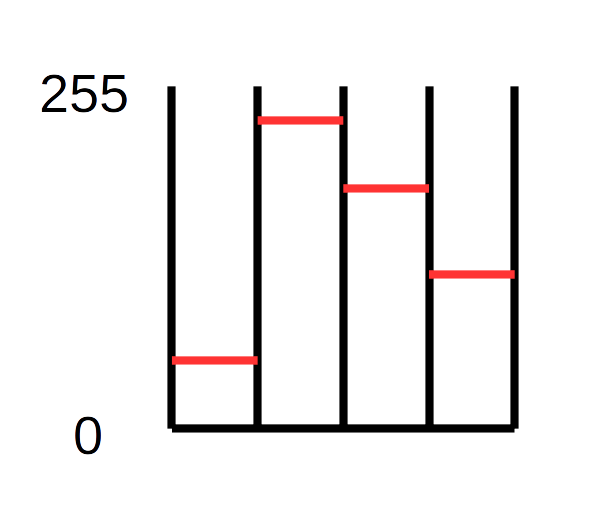
\includegraphics[width=0.5\textwidth]{CCD_ideale_Helligkeit}
  \caption{Helligkeitsverteilung über 4 Pixel bei großer Helligkeit. Der Unterschied zwischen den einzelnen Helligkeitsstufen ist groß.}
  \label{fig:ccd-hell}
\end{figure}

\begin{figure}[h!]
  \centering
    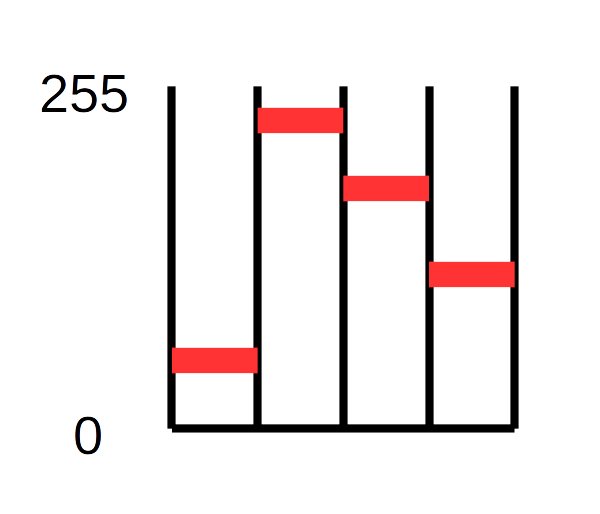
\includegraphics[width=0.5\textwidth]{CCD_Rauschen}
  \caption{Helligkeitsverteilung über 4 Pixel bei großer Helligkeit, inklusive Rauschen (breite der roten Linien). Der Unterschied zwischen den Helligkeitsstufen ist groß, und das Rauschen im Verhältnis zur Helligkeit relativ klein.}
  \label{fig:ccd-rauschen}
\end{figure}

Wenn man nun ein Astrofoto erstellen möchte, stellt sich die Frage, welche Helligkeit ein Bild idealerweise haben sollte. Bei einem zu dunklen Bild (\textit{Abbildung \ref{fig:ccd-dunkel}}) wird der Helligkeitsunterschied zwischen unterschiedlich hellen Regionen zu gering. Schwankt die Helligkeit der Planetenoberfläche beispielsweise um 5\%, und der hellste Bereich erreicht gerade den Farbwert $10$, dann wird die komplette Oberfläche mit einer Helligkeit von 10 abgebildet werden. Die Details der Oberflächenstruktur gehen beim Fotografieren also verloren.

Je größer die maximale Helligkeit ist, desto größer ist der Helligkeitsunterschied im aufgenommenen Bild (\textit{Abbildung \ref{fig:ccd-hell}})

Zusätzlich wird durch eine große Helligkeit der Effekt des Rauschens reduziert, da dieses im Vergleich zu relativen Helligkeit geringer ausfällt, als bei geringen Helligkeiten (\textit{Abbildung \ref{fig:ccd-rauschen}}). Allerdings muss zur Nachbearbeitung der Bilder etwas Platz nach oben gelassen werden. Durch die später angewendeten Schärfe-Filter, werden manche Bereiche des Bildes weiter aufgehellt. Sind die Bilddaten anfangs bereits zu hell, stoßen diese Bereiche bei 255 an, und es gehen wieder Details im Bild verloren. Die ideale Helligkeit ist erreicht, wenn die hellsten Bildbereiche ungefähr 70\% der maximalen Helligkeit erreichen. Das entspricht einem Helligkeitswert von ungefähr 180.

\subsection{Aufnahmemethoden}

\subsubsection{Planeten}

Für die Planetenfotografie der Sternwarte Regensburg steht eine ALccd 5V, sowie eine ALccd 5L-IIm zur Verfügung. Diese Kameras sind besonders auf hohe Bildraten ausgelegt. Da Planeten sehr hell sind, genügen Belichtungszeiten im Millisekunden-Bereich. Idealerweise werden bei der Planetenfotografie über einen Zeitraum von 5 bis 15 Minuten, abhängig vom Planeten, möglichst viele Bilder erstellt.

Diese Bilder werden anschließend zentriert und pixelweise ein Helligkeitsmittelwert berechnet. Da das Rauschen statistisch zufällig verteilt ist, kann durch die Bildung des Mittelwertesbildes das Rauschen minimiert werden. Anschließend kann das Mittelwertbild geschärft werden (\textit{Abbildung \ref{fig:jupiter-bearbeitung}}). Das Schärfen eines Einzelbildes führt dazu, dass das Rauschen das Ergebnisbild dominiert.

\begin{figure}[h!]
  \centering
    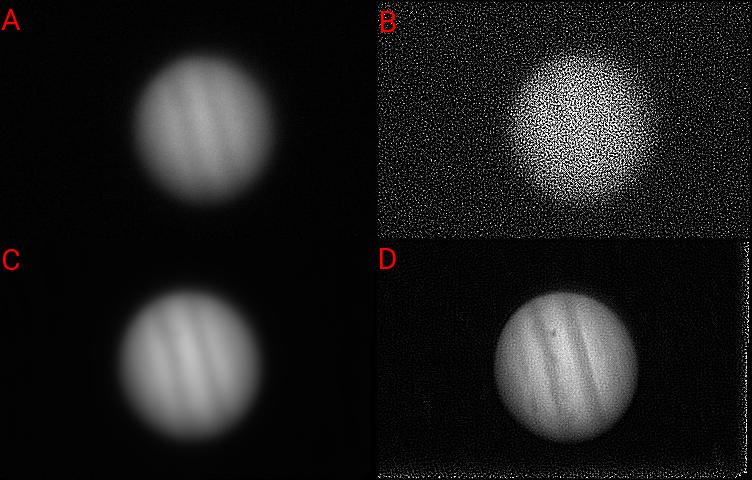
\includegraphics[width=0.9\textwidth]{Jupiter_Bearbeitungsstufen}
  \caption{Jupiter in 4 Bearbeitungsstufen. A ist ein Einzelbild mit deutlich sichtbaren Rauschen. C ist ein Mittelwertbild von vielen Einzelbildern. B ist das geschärfte Ergebnis von A, D das geschärfte Ergebnis von C.}
  \label{fig:jupiter-bearbeitung}
\end{figure}

Das Lichtsammelvermögen, sowie die Brennweite eines Teleskops sind fest durch die Optik vorgegeben. Die Brennweite kann jedoch mit Hilfe von Barlow-Linsen verlängert werden. Um ein ideales Bildergebnis zu erzielen, ist es entscheidend, das vorhandene Licht des Teleskops für die Kamera optimal zu nutzen. 

In Kapitel \ref{sec:abbildung} haben wir gesehen, dass das Abbild mit der Brennweite linear skaliert. Je größer die Brennweite des Teleskops wird, desto größer wird bei konstanter Gesamthelligkeit das Abbild. Das bedeutet, dass auf einzelne Pixel einer Kamera, die sich in der Brennebene befindet, mit zunehmender Bildgröße weniger Licht fällt. Umgekehrt fällt umso mehr Licht auf ein Pixel, je kürzer die Brennweite wird. Je kleiner aber das Abbild auf dem Bildsensor ist, desto weniger Details sind am Ende zu erkennen.

Das Verhältnis aus Helligkeit und Bilddetails sollte optimal gewählt werden. Es ist schon bekannt, dass die Atmosphäre das Auflösungsvermögen auf \ang{;;1} (hier bedeutet das Anführungszeichen Bogensekunde!) begrenzt. Jupiter (oder Saturn mit Ringen) erreicht bei maximaler Erdnähe eine Größe von knapp \ang{;;50}, Mars nur \ang{;;25}. Kleinere Details als \ang{;;1} werden bedingt durch die Erdatmosphäre in der Regel nicht zu sehen sein. Allerdings kann diese Auflösungsbegrenzung durch \href{https://de.wikipedia.org/wiki/Lucky_Imaging}{Lucky Imaging} etwas verbessert werden. Bei der Bearbeitung der Bilder können Programme die Bilder nach Qualität sortieren, und nur einen festgelegten Prozentsatz der besten Bilder weiterverarbeiten. Bei einer Verwendungsrate von 1\% konnte in Versuchen die Seeing-bedingte Auflösung um den Faktor 4 auf ca \ang{;;0,25} verbessert werden \cite{law2006lucky}.

\begin{figure}[h!]
  \centering
    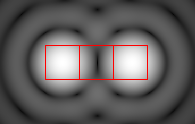
\includegraphics[width=0.5\textwidth]{Pixel_Aufloesung}
  \caption{Es werden mindestens 3 Pixel mit der Größe des Beugungsscheibchen-Radiuses benötigt, um zwei Beugungsscheibchen zu trennen. Quelle: \url{https://en.wikipedia.org/wiki/File:Airy_disk_spacing_near_Rayleigh_criterion.png} (modifiziert)}
  \label{fig:pixel-aufloesung}
\end{figure}

Abhängig davon, ob das Seeing oder die Beugungsbegrenzte Auflösung $\delta_{min}$ des Teleskops die untere Auflösungsgrenze bestimmen, kann für die Pixelgröße einer Kamera eine ideale Brennweite bestimmt werden. Dabei sollte zwischen den Zentren zweier gerade noch zu trennender Beugungsscheibchen mindestens 3 Pixel liegen, um die Helligkeitsunterschiede abbilden zu können.

Daher ergibt sich mit dem Winkeldurchmesser eines Planeten $\delta_p$ eine Auflösung $R$ für den Durchmesser des Planeten:
\begin{equation}
\label{eq:diameter-resolution}
R = 3 \cdot \frac{\delta_p}{\delta_{min}}
\end{equation}
$R$ gibt dabei den Durchmesser in Pixeln an, auf die der Planet abgebildet werden sollte. Für Jupiter mit einem Winkeldurchmesser von $50\si{\SIUnitSymbolArcsecond}$ und einer angepeilten Auflösung von $1"$ würde dies bedeuten, dass das Planetenscheibchen auf dem Fotosensor einen Durchmesser von $150$ Pixeln haben sollte.

Aus der Anzahl der benötigten Pixel für den Planetendurchmesser und der bekannten Pixelgröße $s_{px}$ der Kamera kann nun die Größe des Bildes $B = R \cdot s_{px}$ nach Gleichung \ref{eq:bildgroesse} bestimmt werden.
\begin{equation}
B = G \cdot \frac{b}{g} = R \cdot s_{px}
\end{equation}
In unserem Beispiel mit Jupiter, der 150 Pixel im Durchmesser hat, und einer Pixelgröße von $6\mu m$, bedeutet das, dass das Planetenscheibchen in der Bildebene einen Durchmesser von $900\mu m \approx 1mm$ haben sollte.

Nach Gleichung \ref{eq:b-f} können wir $b = f$ setzen. Wenn wir nun für $R$ Gleichung \ref{eq:diameter-resolution} einsetzen und nach $f$ auflösen, erhalten wir die optimale Brennweite.
\begin{equation}
f = 3 \frac{\delta_p \cdot s_{px} \cdot g}{\delta_{min} \cdot G}
\end{equation}

Die bisherige Rechnung ist allerdings sehr umständlich, da sie für jeden Planeten einzeln durchgeführt werden muss. Mit etwas Geschick ist es möglich, das selbe Ergebnis durch eine etwas einfachere Formel zu erhalten. Für die Gegenstandsweite $g$ und Gegenstandsgröße $G$ gilt die einfache trigonometrische Beziehung (Skizzieren, falls unklar!):
\begin{equation}
\tan\delta_p = \frac{G}{g}
\end{equation}
Durch die Kleinwinkelnäherung erhalten wir die Beziehung:
\begin{equation}
\label{eq:angular-diameter-small-angle}
\delta_p \approx \frac{G}{g}
\end{equation}

Nun rechnen wir quasi rückwärts, um unabhängig vom Planeten die Brennweite des Teleskops zu berechnen. Dazu nehmen wir uns ein \textit{virtuelles Beobachtungsobjekt} zur Hilfe, das wir so klein machen, wie unsere minimale Teleskopauflösung $\delta_{min}$. Wir setzen also $\delta_p = \delta_{min}$, und erhalten nach Gleichung \ref{eq:diameter-resolution} $R = 3$. Wenn wir Gleichung \ref{eq:angular-diameter-small-angle} in Gleichung \ref{eq:bildgroesse} einsetzen und $b \approx f$ zur Hilfe nehmen, erhalten wir
\begin{equation}
B = R \cdot s_{px} = b \frac{G}{g} = b \cdot \delta_{p} = b \cdot \delta_{min} \approx f \cdot \delta_{min}
\end{equation}
Fassen wir zusammen und setzen $R = 3$ ein:
\begin{equation}
3 \cdot s_{px} \approx f \cdot \delta_{min}
\end{equation}
Nach $\delta_{min}$ aufgelöst und mit Gleichung \ref{eq:diameter-resolution} eingesetzt erhalten wir
\begin{equation}
\delta_{min} \approx {\frac{3 \cdot s_{px}}{f}} \approx \sin^{-1}\biggr(1,22 \frac{\lambda}{D}\biggr)
\end{equation}
Nutzen wir nun wieder die Kleinwinkelnäherung, vereinfacht sich die Gleichung zu: 
\begin{equation}
{\frac{3 \cdot s_{px}}{f}} \approx 1,22 \frac{\lambda}{D}
\end{equation}
Zuletzt lösen wir nach $f$ auf:
\begin{equation}
\label{eq:approx-brennweite}
f \approx \frac{3 \cdot D \cdot s_{px}}{1,22 \cdot \lambda}
\end{equation}

\noindent\fbox{\parbox{\textwidth}{\textbf{Zusammenfassung:} Gleichung \ref{eq:approx-brennweite} beschreibt die ungefähre ideale Brennweite abhängig von der Pixelgröße $s_{px}$ einer Kamera, der Wellenlänge $\lambda$ und der Teleskopöffnung $D$. Das Ergebnis ist jedoch unabhängig vom fotografierten Planeten.}}

\begin{table}
\begin{center}
\begin{tabular}{|c|c|c|}
\hline
Kamera & Pixelgröße $s_{px}$ & Maximale Auflösung \\
\hline
ALccd 5V & $\SI[output-product = \times]{6 x 6}{\mu\metre}$ & $\SI[output-product = \times]{752 x 480}{px}$\\
ALccd 5L-IIm & $\SI[output-product = \times]{3,75 x 3,75}{\mu\metre}$ & $\SI[output-product = \times]{1280 x 960}{px}$\\
\hline
\end{tabular}
\caption{Technische Daten der Planetenkameras der Sternwarte Regensburg.}
\label{tbl:kameras}
\end{center}
\end{table}

Unter guten Bedingungen können mit den Teleskopen der Sternwarte Regensburg mit Hilfe von Lucky Imaging vielleicht Auflösungen in der Größenordnung von \ang{;;0,5} erreicht werden. Dazu wird allerdings ein Teleskop mit einer Öffnung von $\SI{300}{\mm}$ benötigt. In dieser Größe stehen in der Sternwarte nur Spiegelteleskope zur Verfügung, die stärkere Bildfehler als der apochromatische Refraktor besitzen.
Nach \ref{tbl:kamerabrennweiten} sollte die Brennweite des Refraktors von $\SI{2250}{\mm}$ ungefähr verdoppelt werden. Deswegen setzen wir eine 2x-Barlowlinse ein.

\begin{table}
\begin{center}
\begin{tabular}{|c|c|c|}
\hline
Kamera & $\delta_{min} = \ang{;;1}$ & $\delta_{min} = \ang{;;0.5}$\\
\hline
ALccd 5V & $f \approx \SI{3850}{\mm}$ & $f \approx \SI{7710}{\mm}$\\
ALccd 5L-IIm & $f \approx \SI{2410}{\mm}$ & $f \approx \SI{4820}{\mm}$ \\
\hline
\end{tabular}
\caption{Ideale Brennweiten für die Kameras der Sternwarte bei einer Auflösung abhängig vom Auflösungsvermögen $\delta_{min}$, gültig für die Planeten Jupiter und Saturn.}
\label{tbl:kamerabrennweiten}
\end{center}
\end{table}

\subsubsection{Spektrographie}
Ebenso wie bei der Planetenfotografie, lohnt es sich bei der Spektroskopie nicht, eine zu große Brennweite zu haben. Im Regelfall kann auch weit oberhalb der Auflösungsgrenze gearbeitet werden. Neben dem Auflösungsvermögen des Teleskops gibt es noch ein Auflösungsvermögen des Spektroskops, das unter anderem von der Spaltbreite des Spektrographen abhängt, sowie der Pixelgröße der sich dahinter befindlichen Kamera, beziehungsweise ihres Abstands zum Gitter. \url{https://www.silicann.com/blog/beitrag/spektrale-aufloesung-eklaert/} und \url{https://www.silicann.com/blog/beitrag/spektrometer-aufloesung-vs-sensitivitaet/} bieten weitere Infos zur spektralen Auflösung.

Für die Belichtung gelten bei der Spektroskopie die gleichen Regeln wie bei der Planetenfotografie. Da das Bild aber nicht geschärft wird, darf die Belichtungszeit so gewählt werden, dass die maximale Intensität bei einem Helligkeitswert von 80 \% bis 90\% der maximalen Farbtiefe liegen kann.

Technisch ist es auch möglich, mehrere Bilder zu erstellen und daraus ein Mittelwertbild zu erstellen, um das Rauschen zu reduzieren. Praktischerweise genügt es allerdings häufig schon, über die 10 Pixel der Breite des Spektrums zu mitteln, um das Rauschen deutlich zu reduzieren. Für einfachere Anwendungsfälle genügt es daher, ein einzelnes scharfes Bild des Spektrums zu erzeugen.



\subsubsection{Deep-Sky}
Es steht eine QHY8 CCD-Kamera zur Verfügung. Eine Anleitung ist hier verfügbar: \url{www.qhyccd.com/files/QHY8L\%20user\%20manual.pdf}

\section{Bildaufnahme}
In die Bedienung der Teleskope wird vom Sternwartenpersonal eingewiesen. Wenn etwas unklar ist, bitte immer eines der anwesenden Sternwartenmitglieder fragen.

\textbf{ACHTUNG:} Das Berühren aller optischen Flächen (Linsen, Spiegel, Kameras, Okulare, Filter, etc.) ist unbedingt zu vermeiden!

Alle Daten können zentral auf dem Sternwartenserver gespeichert werden. Auf diesen kann entweder über WLAN oder LAN zugegriffen werden. Die Adresse des Netzlaufwerks ist \url{\\\\192.168.113.2\\sternwarte} (\textit{Abbildung \ref{fig:laufwerk}}). Die Daten können im Ordner \textit{Astro-Rohdaten} gespeichert werden. Für jede Projektgruppe sollte dabei ein eigener Ordner angelegt werden. Es ist auf eine sinnvolle Benennung und Sortierung der aufgenommenen Daten zu achten, damit anschließend die Bearbeitung gut funktioniert.

\begin{figure}[h!]
  \centering
    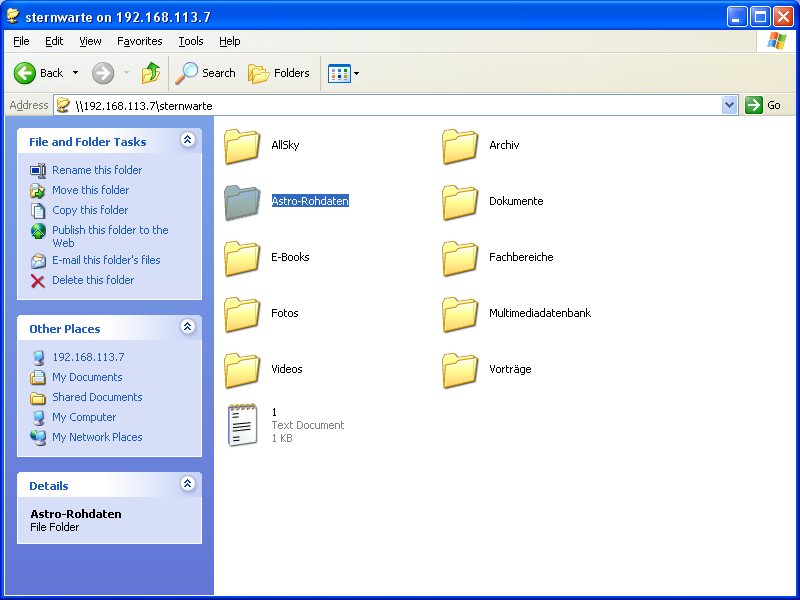
\includegraphics[width=0.9\textwidth]{Laufwerk}
  \caption{Sternwartenlaufwerk}
  \label{fig:laufwerk}
\end{figure}


\subsection{ALCCD 5V}
Zur Fotografie mit der ALCCD 5V wird die Software QGVideo/32, sowie der Treiber benötigt. Die Programme befinden sich auf dem Sternwarten-Laufwerk im Ordner \textit{Astro-Rohdaten\textbackslash Programme\textbackslash Alccd5v CD}.

\subsubsection{Schritt für Schritt Anleitung}

\begin{figure}[h!]
  \centering
    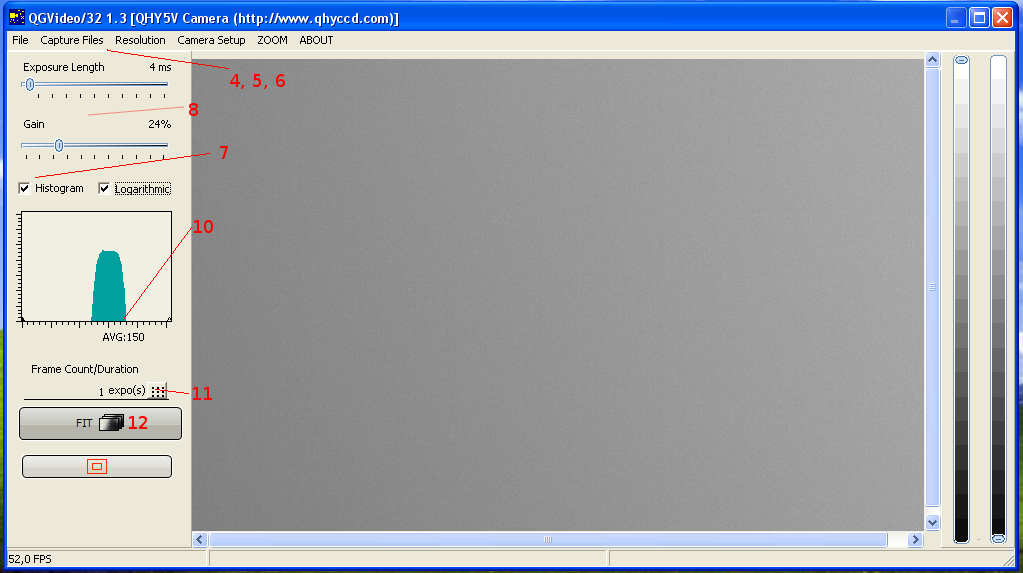
\includegraphics[width=0.9\textwidth]{QGVideo32-annotiert}
  \caption{QGVideo32}
  \label{fig:qgvideo32}
\end{figure}

\begin{enumerate} 
\item Objekt / Planet im Teleskop mit Okular möglichst genau ohne Zenitspiegel zentrieren.
\item Kamera an Laptop / PC anschließen.
\item QGVideo/32 starten
\item Menüpunkt \textit{Capture Files \textgreater Set Capture Location} auswählen, und als Speicherordner C:\textbackslash Aufnahmen\textbackslash [Objektname-Datum]\textbackslash
\item Menüpunkt \textit{Capture Files \textgreater Set Capture Filename} auf Beginn der Uhrzeit der aktuellen Belichtungsrunde setzen
\item Im Menüpunkt \textit{Capture Files \textgreater Set Capture Format} AVI auswählen
\item Histogramm aktivieren und auf Logarithmisch stellen.
\item Zunächst Gain und Exposure Length hoch drehen und schauen, ob ein unscharfer Ring zu sehen ist. Ggf etwas an der Kamera wackeln, um zu sehen, wo der Planet ist. Sobald der Planet gefunden ist, mit der Montierungssteuerung zentrieren, und fokussieren. Dabei Gain und Exposure Length nach Bedarf wieder herabregeln. Im Menüpunkt \textit{Resolution} 376x240 (subframe) auswählen, sobald der Planet genau genug zentriert ist.
\item Zeit lassen, um den Fokuspunkt genau zu finden.
\item Gain auf maximal 50\% drehen, lieber niedriger, und die Exposure Length so regeln, dass das Histogramm bei einer Helligkeit von 180 aufhört.
\item \textit{Frame Count/Duration} auf Sekunden stellen. Für Jupiter dürfen für alle Farbkanäle nicht mehr als 5 Minuten belichtet werden, bei Mars und Saturn nicht mehr als 15 Minuten.
\item Für jeden Farbkanal auf den Aufnahme-Knopf drücken.
\item Nach Aufnahme der Farbkanäle die aufgenommenen Dateien aussagekräftig umbenennen und auf den Datei-Server verschieben.
\end{enumerate}


\subsection{ALCCD 5L-IIm}
Zur Fotografie mit der ALCCD 5L-IIm wird die Software EZPlanetary, sowie der Treiber benötigt. Die Programme befinden sich auf dem Sternwarten-Laufwerk im Ordner \textit{Astro-Rohdaten\textbackslash Programme\textbackslash Alccd5L-IIm CD}.

\subsubsection{Schritt für Schritt Anleitung}

\begin{figure}[h!]
  \centering
    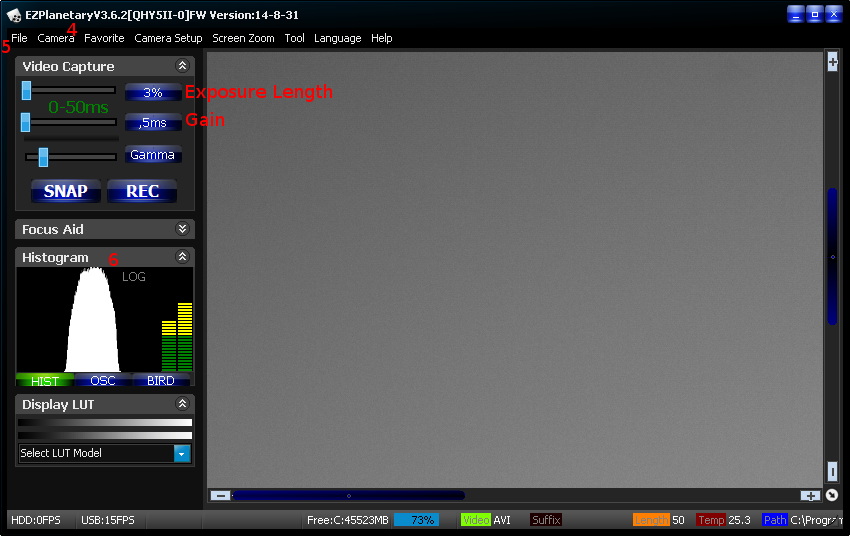
\includegraphics[width=0.9\textwidth]{EZPlanetary-annotiert}
  \caption{EZPlanetary}
  \label{fig:ezplanetary}
\end{figure}

\begin{enumerate} 
\item Objekt / Planet im Teleskop mit Okular möglichst genau ohne Zenitspiegel zentrieren.
\item Kamera an Laptop / PC anschließen.
\item EZPlanetary starten
\item Menüpunkt \textit{Camera \textgreater QHY5L-II} die Auflösung 1280x960 wählen.
\item Menüpunkt \textit{Files \textgreater Video Record Options} auswählen, und als Speicherordner C:\textbackslash Aufnahmen\textbackslash [Objektname-Datum]\textbackslash setzen, Videoformat auf AVI. Aufnahmelänge auf Duration und Schieber auf Skala entsprechend anpassen. Für Jupiter dürfen für alle Farbkanäle nicht mehr als 5 Minuten belichtet werden, bei Mars und Saturn nicht mehr als 15 Minuten.
\item Histogramm aktivieren und auf Logarithmisch stellen.
\item Zunächst Gain und Exposure Length hoch drehen und schauen, ob ein unscharfer Ring zu sehen ist. Ggf etwas an der Kamera wackeln, um zu sehen, wo der Planet (Objekt) ist. Sobald der Planet gefunden ist, mit der Montierungssteuerung zentrieren, und fokussieren. Dabei Gain und Exposure Length nach Bedarf wieder herabregeln. Im Menüpunkt \textit{Camera \textgreater} 320x240 auswählen, sobald der Planet genau genug zentriert ist.
\item Zeit lassen, um den Fokuspunkt genau zu finden.
\item Gain auf maximal 50\% drehen, lieber niedriger, und die Exposure Length so regeln, dass das Histogramm bei einer Helligkeit von 180 aufhört. Die Skala am rechten Rand des Histograms darf nicht in den roten Bereich kommen, sondern sollte am oberen Ende des gelben Bereichs sein.
\item Für jeden Farbkanal auf den REC-Knopf drücken.
\item Nach Aufnahme der Farbkanäle die aufgenommenen Dateien aussagekräftig umbenennen und auf den Datei-Server verschieben.
\end{enumerate}

\subsection{Spektrograph und QHY8}
Anleitungen zu den Geräten finden sich im Netzlaufwerk der Sternwarte im Ordner Anleitungen, sowie auf \url{https://stw-r.de/manuals/}.

Bei der Montage des DADOS und der QHY8 ist darauf zu achten, dass das Spektrum möglichst parallel zur langen Seite des CCD-Chips projiziert wird. Das reduziert die nötige Rotation des Spektrums bei der Bearbeitung.

Für die Aufnahme der Spektren wird die QHY8 zusammen EZCap verwendet. Wichtig ist, dass das Bild nach jeder Aufnahme gespeichert wird, da sonst das Programm abstürzt.

Zur späteren Eichung der Wellenlängen sollte zunächst ein Stern mit deutlichen H-alpha, H-beta und H-gamma Linien aufgenommen werden. Anschließend sollte der Aufbau nicht mehr verändert werden und die eigentlichen Messobjekte aufgenommen werden. Außerdem kann ein heller Stern (oder die Laborlichtquelle) dazu genutzt werden, die Kamera in den Fokus des Spektrographen zu bringen.

Bei der Belichtung eines Sterns sollte der mittlere Spalt verwendet werden. Er ist mit $25\mu m$ Breite am schmalsten und hat die beste spektrale Auflösung. Je mittiger in der Linie fotografiert wird, desto geringer ist die Bildwölbung des resultierenden Fotos und desto präziser ist das Spektrum auswertbar.

\section{Bildbearbeitung}
\subsection{Planeten}
Die Bildbearbeitung erfolgt in mehreren Schritten. Die Benutzung der einzelnen Programme ist in jeweils einem eigenen Abschnitt erklärt.
\begin{enumerate}
\item Mittelwert-Bild berechnen mit Autostakkert \\ \url{http://www.autostakkert.com/}
\item Mittelwert-Bild schärfen mit Giotto \\ \url{http://www.giotto-software.de/giotto.htm}
\item LRGB-Mittelwertbilder mit Fitswork zu einem Bild zusammensetzen \\ \url{http://www.fitswork.de/software/} \\
Da Fitswork als Luminanzbild keine RGB-Skala verarbeiten kann, muss vorher das Luminanzbild beispielsweise mit \href{http://gimp.org}{GIMP} über den Menüpunkt \textit{Farben \textgreater Entsättigen} entsättigt werden.
\end{enumerate}
\subsubsection{Autostakkert}
Das Programm Autostakkert ist in der Lage, sowohl aus AVIs von Planeten als auch von Oberflächen sehr schnell ein Mittelwertbild zu berechnen.

\begin{figure}[h!]
  \centering
    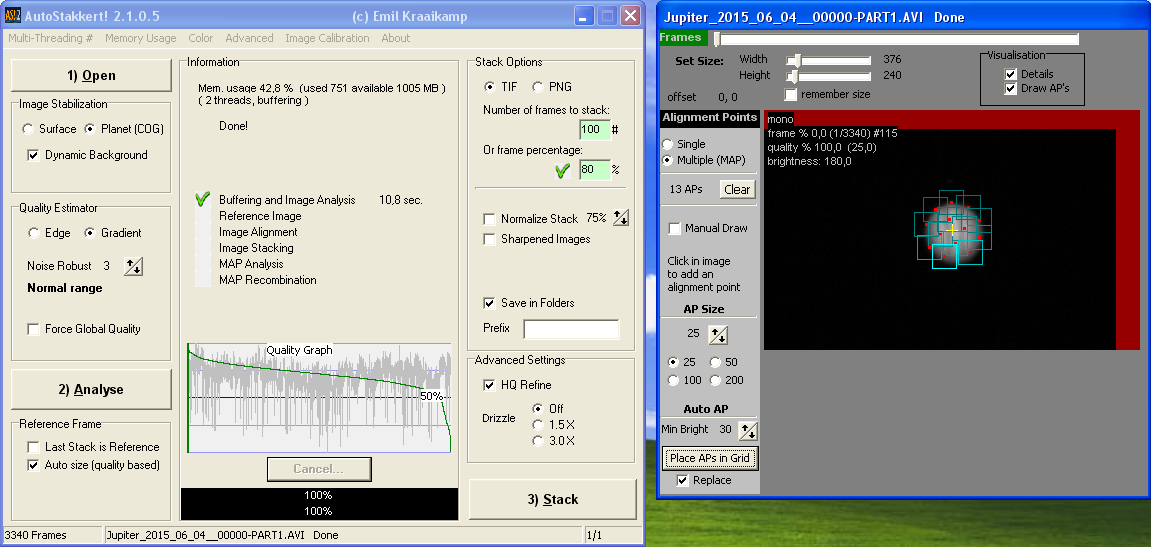
\includegraphics[width=0.9\textwidth]{AutoStakkert}
  \caption{Das Programm AutoStakkert zum Berechnen eines Mittelwertbildes.}
  \label{fig:autostakkert}
\end{figure}

\begin{enumerate}
\item AutoStakkert öffnen
\item \textit{1) Open} klicken und eine Video-Datei auswählen.
\item Planet oder Surface auswählen, abhängig vom bearbeiteten Objekt.
\item \textit{2) Analyze} klicken
\item Anhand der Qualitätskurve muss jetzt die Anzahl oder den Prozentsatz der zu mittelnden Bilder in der Box \textit{Stack Options} (rechts oben) festgelegt werden. Es sollten mindestens 100 Bilder gemittelt werden. Dabei sollte aber die durchschnittliche Qualität der genutzten Bilder möglichst hoch sein.
\item Im Bild-Fenster den Button \textit{Place APs in Grid} (rechtes Fenster, links unten) klicken.
\item \textit{3) Stack} klicken.
\item AutoStakkert erstellt im selben Ordner, in dem das Video liegt, einen Unterordner mit dem Namen \textit{AS\textunderscore pXY\textunderscore Multi} und legt darin das Mittelwertbild ab. Nach jedem Durchlauf mit AutoStakkert sollte die darin befindliche Datei sofort aussagekräftig umbenannt werden. Beispiel: \textit{ Jupiter\textunderscore 1\textunderscore L.tif}
\end{enumerate}

\subsubsection{Giotto}
Giotto enthält einen sehr guten Satz an Schärfungsfiltern. Die Arbeitsumgebung von Giotto ist etwas ungewöhnlich und besteht aus 4 Arbeitsbereichen: den Puffern A bis D. Insgesamt können also maximal 4 Bilder gleichzeitig geöffnet sein. Nachdem ein Bild mit dem \textit{Datei \textgreater Bild laden ...} Dialog geöffnet wurde, kann es mit dem Dialog \textit{Bearbeiten \textgreater Schärfen und Filtern} geschärft werden. Die Ergebnisse des Schärfungsprozesses können dann in die Puffer B bis D geladen, und so unterschiedliche Ergebnisse verglichen werden.

\begin{figure}[h!]
  \centering
    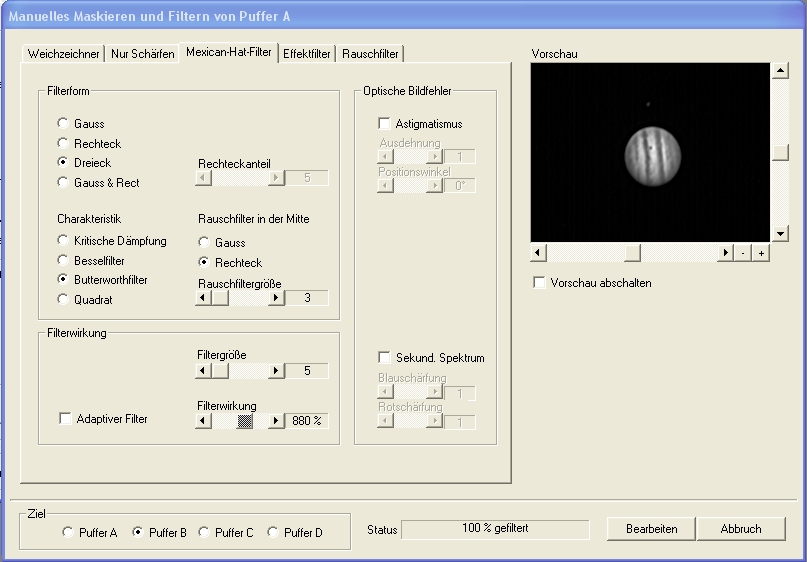
\includegraphics[width=0.9\textwidth]{Giotto-Filter}
  \caption{Das Programm Giotto enthält sehr gute Schärfungsalgorithmen. Hier ist eine sinnvolle Vorauswahl für die Schärfung von Planeten zu sehen.}
  \label{fig:giotto}
\end{figure}

Zum Schärfen eignet sich insbesondere der Reiter \textit{Mexican-Hat-Filter} aus dem \textit{Schärfen und Filtern}-Dialog. Der Abbildung \ref{fig:giotto} ist eine sinnvolle Vorauswahl an Filtereinstellungen zu entnehmen. An den Filtereinstellungen kann viel ausprobiert werden, um ein optimales Ergebnis zu erzielen.

Das fertig geschärfte Bild muss dann über den \textit{Datei \textgreater Bild speichern ...}-Dialog gespeichert werden. Das vorige ungeschärfte Bild sollte bei nicht überschrieben werden, da es eventuell für einen neuen Schärfungsdurchgang benötigt wird. Es ist wieder auf eine aussagekräftige Namensgebung zu achten. Beispiel: \textit{Jupiter\textunderscore 1\textunderscore L\textunderscore geschaerft.png}

\subsubsection{Fitswork}

Mit Fitswork können die Schwarz-Weiß-Bilder der einzelnen Farbkanäle zu einem RGB-Bild zusammengefügt werden. Zunächst müssen dazu die geschärften Bilder des R-, G- und B-Kanals geladen werden. In jedem der Bilder kann man mit Links-Klick einen gelben Kasten um den Planeten ziehen, damit das Programm den Planeten besser finden kann. Anschließend wählt man im Menü \textit{Bilder Kombinieren \textgreater 3 s/w Bilder zu RGB Bild (mit Verschiebung)}. 

Wahrscheinlich werden die Farblayer noch nicht korrekt aufeinander ausgerichtet sein. Deswegen kann man das Ergebnis noch mit dem Menüpunkt \textit{Bearbeiten \textgreater Farblayer zurechtrücken} verbessern. Dieser Schritt kann so oft wiederholt werden, bis die Farblayer korrekt ausgerichtet sind.

Das finale RGB Bild kann jetzt zur Sicherheit wieder gespeichert werden. Letztendlich wird jetzt noch der Luminanzkanal über das RGB-Bild gelegt, um mehr Details aus dem Bild heraus zu holen. Dazu muss das Luminanz-Bild entsättigt sein, da Fitswork mit RGB-Farbwerten bei einem Luminanz-Bild nicht umgehen kann. Das kann beispielsweise mit \href{http://gimp.org}{GIMP} über den Menüpunkt \textit{Farben \textgreater Entsättigen} erledigt werden.

Das entsättigte Luminanz-Bild wird zunächst wieder über den \textit{Datei \textgreater Öffnen}-Dialog geöffnet. Zum Erstellen des LRGB-Bildes wird nun der Menüpunkt \textit{Bilder Kombinieren \textgreater L+RGB Bild kombinieren nicht skaliert} gewählt.

Eine Fein-Optimierung des Bildes kann jetzt noch mit den verschiedenen Bildbearbeitungsoptionen von Giotto oder Gimp geschehen.

\subsection{Spektren}
Aufgenommene Spektren müssen zunächst so rotiert werden, dass das aufgenommene Spektrum möglichst horizontal im Bild liegt. Das kann beispielsweise zur Hilfenahme des Werkzeugs \textit{Ebene} \textgreater \textit{Transformieren} \textgreater \textit{beliebige Rotation} von GIMP geschehen.

Anschließend kann der Bereich des Spektrums ausgeschnitten werden. Dabei sollte das komplette Breite des Bildes mit ausgeschnitten werden, damit die verschiedenen Aufgenommen Spektren später verglichen werden können. Das bedeutet, dass die Zuordnung von Pixel zu Wellenlänge in allen Spektren gleich bleibt. Das resultierende Bild sollte ungefähr 10 Pixel hoch und 3328 Pixel breit sein.

Die Helligkeiten können nun vertikal gemittelt werden, um das Rauschen zu reduzieren. Dazu kann ein kleines Python-Programm genutzt werden, welches frei heruntarladbar ist: \href{https://github.com/svenseeberg/evaluate-spectrum}{https://github.com/svenseeberg/evaluate-spectrum}

Die resultierende CSV-Datei kann dann mit SciDavis oder einem anderen Programm geöffnet und weiter verarbeitet werden.

\section{Auswertung}
\subsection{Altersbestimmung der Mondoberfläche}

\noindent\fbox{\parbox{\textwidth}{\textbf{Hinweis:} Die Berechnung des Oberflächenalters ist nur eine grobe Näherung. Dafür gibt es drei Ursachen: Erstens ist die Bestimmung eines Flächenelements von genau $\SI{10000}{km^2}$ schwierig. Wir benutzen hier nur eine grobe Näherung. Zweitens ist das Ablesen des Alters aus dem Diagramm \ref{fig:crateringrate} unpräzise. Und drittens sind nur vergleichsweise wenige Messpunkte für das Alter der Mondoberfläche vorhanden, so dass große statistische Abweichungen möglich sind.}}

Anhand der Kraterdichte kann das Alter der Mondoberfläche bestimmt werden. Die Kraterdichte ist die Anzahl der Einschlagskrater pro Quadratkilometer. Um ein Rechteck mit bekannter Seitenlänge über das Bild zu legen, muss zunächst der Maßstab berechnet werden. Hierzu können 2 verschiedene Wege genutzt werden: Entweder kann mittels Mondatlas die Größe eines Referenzkraters in einer gewählten Region bestimmt werden. Oder es wird über die optischen Eigenschaften des Teleskops und der Kamera der Abbildungsmaßstab berechnet. Eine genaue Bestimmung des Kraters auf einem Mondatlas ist die wesentlich präzisere Methode.

Nach \ref{eq:bildgroesse} ist die Bildgröße des Mondes leicht zu berechnen. Das Bild entspricht dem Gesamtdurchmesser des Mondes von annähernd $d = \SI{3500}{km}$. Die Größe der Kamerachips oder die Pixelgröße ist bekannt. Der Maßstab $M$ in Kilometer pro Pixel kann berechnet werden durch

\begin{equation}
M = \frac{s_{px}}{B} \cdot \SI{3500}{km}
\label{eq:masstab}
\end{equation}

VORSICHT: Dieser Maßstab bezieht die Wölbung des Mondbildes noch nicht mit ein. Der Maßstab ist daher nur in einem kleinen Bereich in der Mitte des Mondes annähernd richtig, beziehungsweise entlang eines Kreisbogens, deren Mittelpunkt im Mondzentrum liegt.

\begin{figure}[h!]
  \centering
    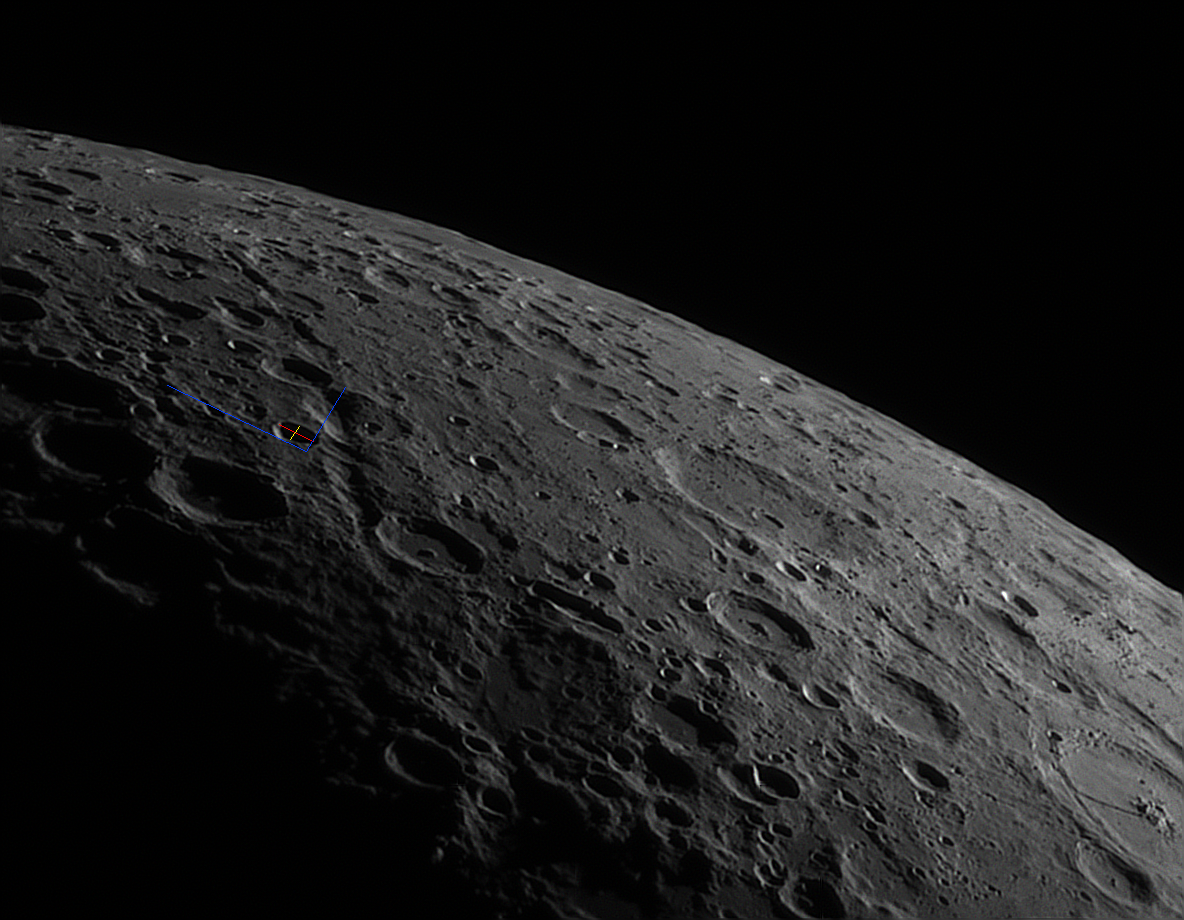
\includegraphics[width=1\textwidth]{Mondkrater}
  \caption{Die Mondoberfläche aufgenommen mit der ALccd 5L-IIm und dem Refraktor. Bei einer Brennweite von $f = \SI{2,25}{m}$ ist das Bild ungefähr $B \approx \SI{2}{cm}$ groß. Entlang der roten Linie (große Achse, rote Linie) hat der Krater einen Durchmesser von $39,4 px$. Das entspricht nach Gleichung \ref{eq:masstab} einer Distanz von $\SI{25,5}{km}$. Die kleine Achse (gelb) hat eine Länge von $\SI{19,2}{px}$. Eine Region mit $\SI{10000}{km^2}$ hat hat daher eine Kantenlänge von $\SI{154,4}{px}$ in tangentialer Richtung, sowie $\SI{75,3}{px}$ in radialer Richtung (blau).}
  \label{fig:mondkrater}
\end{figure}

Wir nehmen an, dass die meisten Krater näherungsweise kreisrund sind. Deswegen kann die - nur durch die optische Verzerrung existierende - lange Halbachse in Pixeln gemessen und mit dem Maßstab multipliziert werden. Das Verhältnis aus kleiner und großer Halbachse ergibt dann den Maßstab in radialer Richtung.

\begin{figure}[h!]
  \centering
    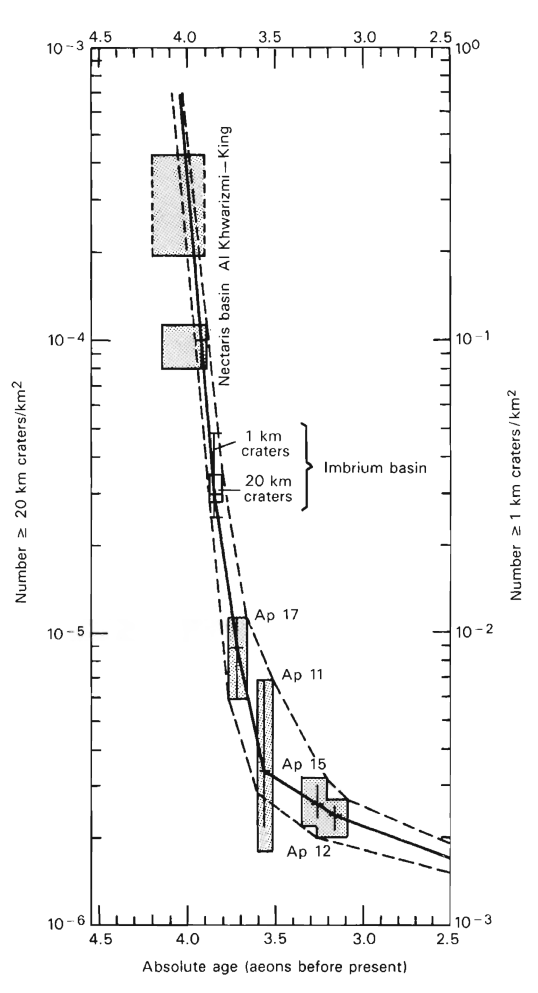
\includegraphics[width=0.5\textwidth]{Altersbestimmung_Mondoberflaeche}
  \caption{Alter der Mondoberfläche in Abhängigkeit von der Kraterdichte. Quelle: \url{http://www.lpi.usra.edu/publications/books/geologyTerraPlanets/GeologyTerrestrialPlanets.pdf}}
  \label{fig:crateringrate}
\end{figure}

Anschließend kann ein Rechteck mit der Kantenlänge $\SI{100}{km}$ definiert werden, in dem die Krater gezählt werden können. Nur Krater mit einem Durchmesser von mehr als $\SI{20}{km}$ dürfen gezählt werden. Die Zahl muss anschließend auf Krater pro Quadratkilometer normiert werden. Mit dieser Zahl kann aus Abbildung \ref{fig:crateringrate} das Alter der Region bestimmt werden.

\bibliography{references1.bib}{}
\bibliographystyle{plain}

\end{document}